\documentclass{standalone}
\usepackage{tikz}
\usepackage{pict2e}

\DeclareRobustCommand{\slashcirc}{{\mathpalette\doslashcirc\relax}}

\makeatletter
\newcommand\doslashcirc[2]{%
  \sbox\z@{$#1\m@th\circ$}%
  \setlength\unitlength{\wd\z@}
  \begin{picture}(1,1)
  \roundcap
  \put(0,0){\box\z@}
  \put(0,0){\line(1,1){1}}
  \end{picture}%
}
\makeatother


\begin{document}

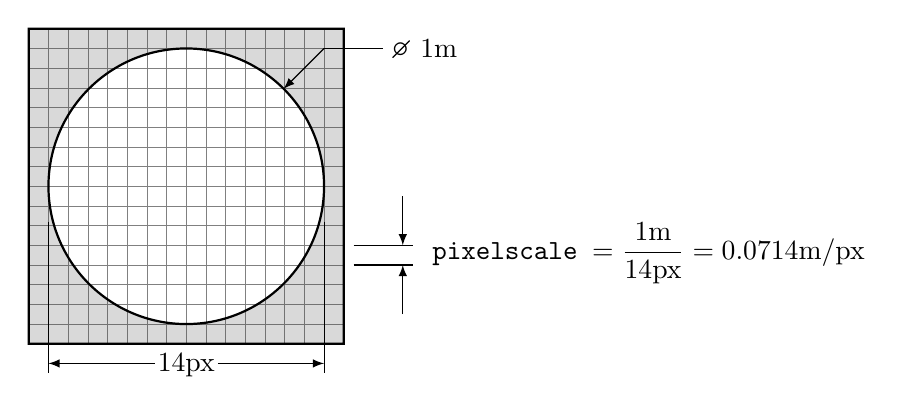
\begin{tikzpicture}


\draw [very thin, gray, step=0.25] (-2,-2) grid +(4,4);
\draw [thick, fill=darkgray, fill opacity=0.2, even odd rule] (-2,-2) -- (2,-2) -- (2,2) -- (-2,2) -- cycle (0,0) circle[radius=1.75]; 

\draw[latex-] (-1.75,-2.25) -- (-0.4,-2.25);
\draw[-latex] (0.4,-2.25) -- (1.75,-2.25);

\draw (-1.75,-0.45) -- (-1.75,-2.375);
\draw (1.75,-0.45) -- (1.75,-2.375);
\node [below] at (0,-2) {14\mbox{px}};

\draw[latex-] (1.237,1.237) -- (1.75,1.75);
\draw (1.75,1.75) -- (2.5,1.75);
\node[right] at (2.5,1.75)  {\large$\slashcirc$ \normalsize$1\mbox{m}$};

%\draw[-latex] (1.875,-1.625) -- (1.875,-1);
%\draw[latex-] (1.875,-.75) -- (1.875,-0.125);
%\draw (1.875,-0.125) -- (2.375,0.375);

\draw (2.125,-1) -- (2.875, -1);
\draw (2.125,-0.75) -- (2.875, -0.75);
\draw[-latex] (2.75,-1.625) -- (2.75,-1);
\draw[latex-] (2.75,-.75) -- (2.75,-0.125);

\node[align=left, right] at (3, -0.85) {\texttt{pixelscale }$=\displaystyle \frac{1\mbox{m}}{14\mbox{px}}=0.0714 \mbox{m/px}$};
%2.5, 0.125

\end{tikzpicture}
\end{document}
